\chapter{Hyperparameters}
\section{K-Means}
For selecting the appropriate amount of clusters, we used an "elbow" plot in combination with the silhouette score.
\begin{enumerate}
  \item Dataset 1: 4 clusters (see figure: \ref{hyperparameters:k-means-dataset1})
  \item Dataset 2: TODO
  \item Dataset 3: TODO
\end{enumerate}
\begin{figure}
  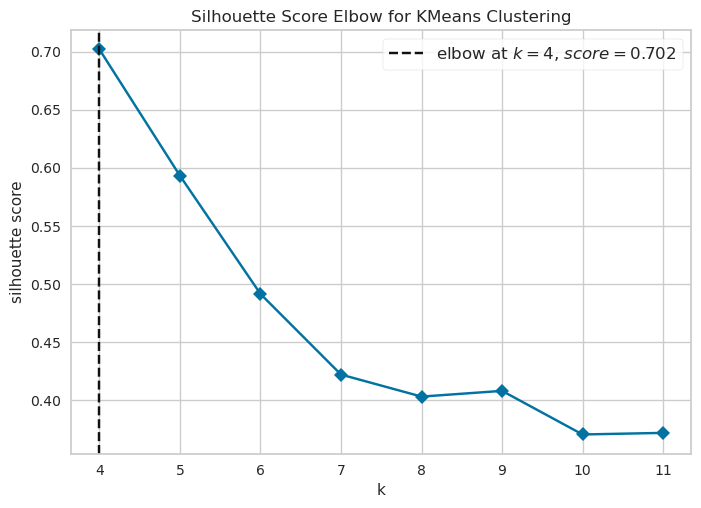
\includegraphics{Appendix/parameter-selection/selecting-k.png}
  \caption{Selecting the $k$ for K-Means for dataset 1 using the "elbow plot" using section \ref{theory:kmeans}}
  \label{hyperparameters:k-means-dataset1}
\end{figure}
\section{DBSCAN}
For the selection of the appropriate epsilon, we used the k-distance plot.
\begin{enumerate}
  \item Dataset 1: 0.9 epsilon (see figure: \ref{hyperparameters:DBSCAN-dataset1})
  \item Dataset 2: TODO
  \item Dataset 3: TODO
\end{enumerate}

\begin{figure}
  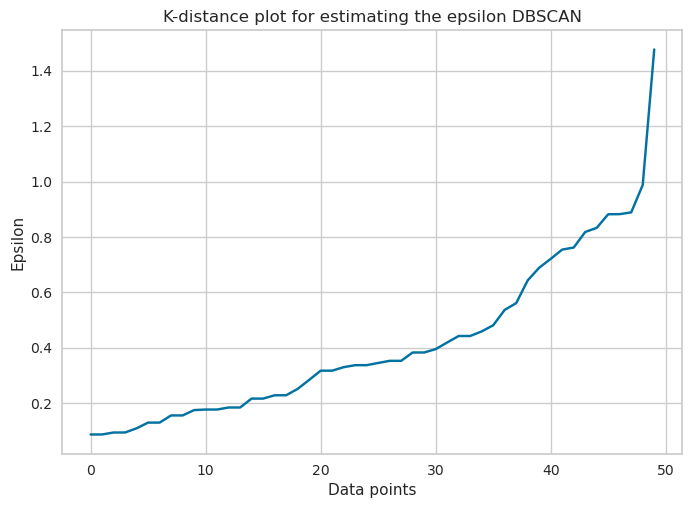
\includegraphics{Appendix/parameter-selection/selecting-eps.png}
  \caption{Selecting the $\epsilon$ for DBSCAN for dataset 1 using the "k-distance plot" using section \ref{theory:clustering-dbscan}}
  \label{hyperparameters:DBSCAN-dataset1}
\end{figure}